%%% Made of Tiny Robots
%%% An Investigation of the Ecology of Responsive Environments
%%%
\chapter{An Ontology of Responsive Environments}
\label{ch:ontology}
%
As we enter the age of ubiquitous computing our relationship with our artifact ecology is changing. 
There are several factors to these changes: we have new ways to fabricate artifacts; we have new ways of relating to artifacts; and our artifacts increasingly perform tasks that were once the exclusive domain of people.
To facilitate a discussion of these changes we here describe the components of these responsive ecologies in more detail, and coin several terms to refer to these components.
In Section~\ref{sec:kinds_of_artifacts} we suggest some categories for distinguishing different kinds of artifacts according to their purpose and means of production.
In Section~\ref{sec:roles} we discuss how these categories help to structure the roles we can play in relation to the production and use of artifacts.

In Section~\ref{sec:artifact_ecologies} we describe the responsive artifact ecologies introduced in Chapter~\ref{ch:intro} in more detail. 
We suggest that one of the key distinctions between these different ecologies is the roles that are available for members of each society to play; ecologies structured around more transparent technological mechanisms and more reconfigurable artifacts will present more opportunities for people to adopt roles that shape the behavior of their environment. 
Of particular interest is what we are calling a robunculi ecology: manufacturing is focused on producing robotic kits of parts rather than devices that perform a single role; these kits can either be assembled, or can self-assemble, into a variety of forms on demand. 

To promote the potential for involving a wide spectrum of society in design roles we develop our ontology of robunculi further in Section~\ref{sec:robunculi_ontology}. 
We examine in more detail the roles people can play in producing and using robunculi, and the interaction methods available for people adopting various roles.


\section{Kinds of Artifacts}
\label{sec:kinds_of_artifacts}
%
By embedding computation in artifacts we can expand both the purposes they can serve and our means of producing new artifacts. 
We have developed some terminology to describe artifacts in both of these axes. 
Together the categories of production and purpose help to determine the roles we can play in relating to a given artifact.

\subsection{Artifact Production Typologies}
%
In a popsicle ecology we are used to purchasing packaged preconfigured devices. As illustrated in Figure~\ref{fig:hardware_venn} there are several ways a device can be implemented in a responsive environment. 

\begin{figure}[]
  \centering
    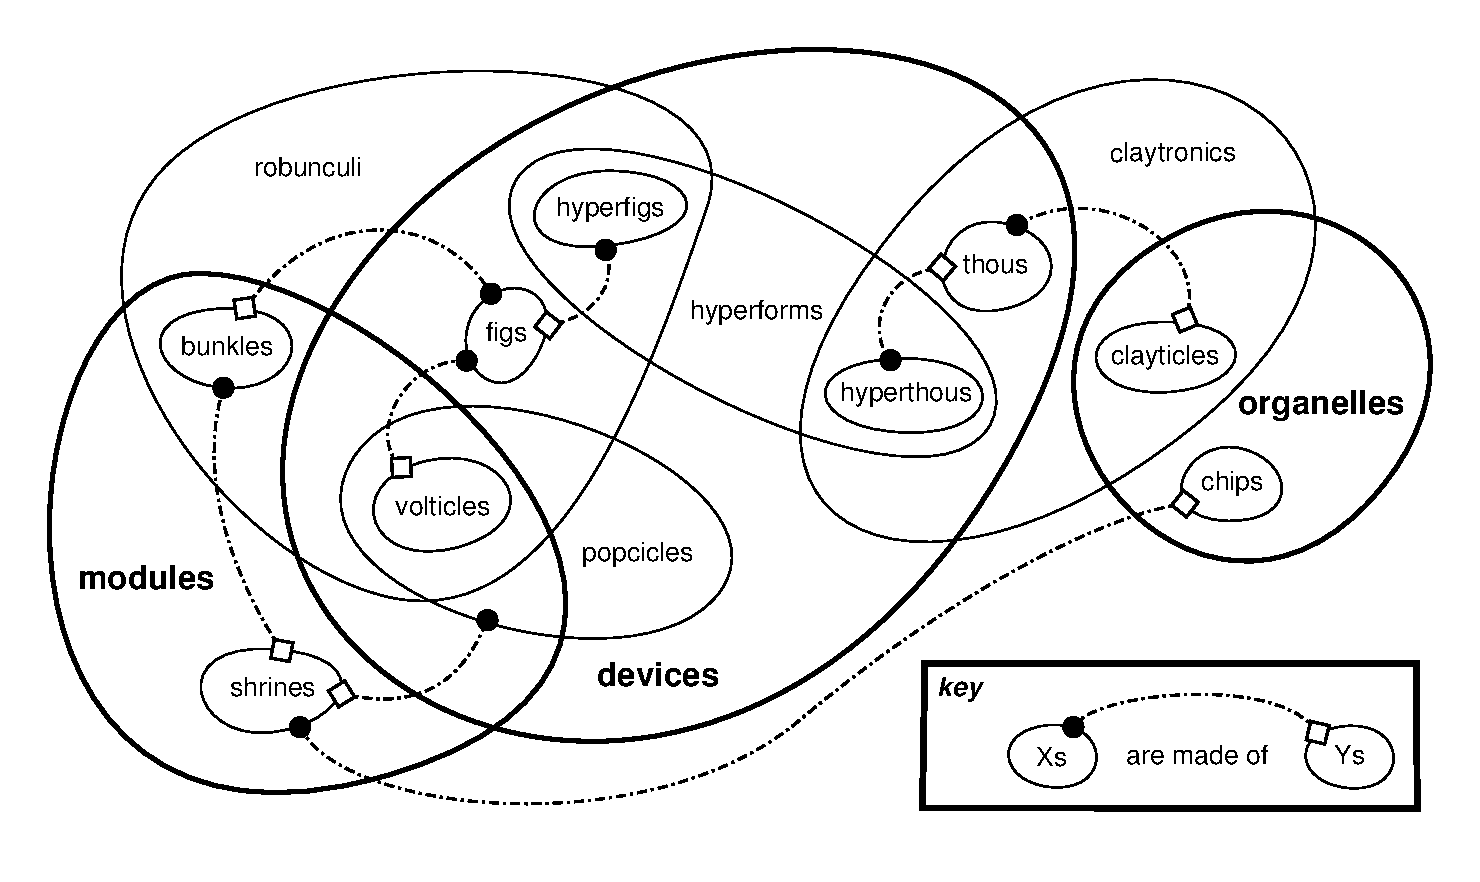
\includegraphics[width=140mm]{hardware_venn.pdf}
  \caption{Venn diagram of computational artifact hardware categories.}
  \label{fig:hardware_venn}
\end{figure}

Two important factors in the production of responsive hardware are scale and tooling. 
At the smallest end are chips, analog electronic components, sensors and actuators. 
We will refer to this group collectively as \emph{organelles}, after the tiny machines that power biological cells; these components are generally produced in high volumes in and require expensive, technologically sophisticated tooling usually found in factories. 
Even supposedly \textbf{open hardware} systems are built around these closed organelles. 

At the next scale are modules that package these organelles to make them more accessible to spoke developers (for example an \textbf{Arduino} board), or to present a tangible interface (like our Posey kit). 
(The Arduino is an example of a \emph{shrine}, a computing module that can, among other things, allow a device to communicate with idols.) 
This stage of production can take place at a sophisticated local fab shop (with tools such as a \textbf{pick-and-place}) but often takes place in a more traditional factory because of the economic advantages of scale.

Popsicles are generally manufactured as a monolithic design including the necessary organelles on a custom circuit board, and sandwiched inside of a factory-produced case. 
Spoke and robunculi ecologies make use of modules to lower the barrier to device design. 
Sharing high-level components reduces the amount of technological knowledge required to create and customize devices.
Open hardware circuit modules abstract away from the complexity of organelles and electronics, and are generally accompanied by online code samples and tutorials. 
Open hardware designs for cases and mechanical components can also be downloaded, customized and then fabricated with \textbf{rapid prototyping}%
\footnote{Some examples of rapid prototyping technologies commonly available at local fab shops are \textbf{fused deposition modeling (FDM)} 3D printers and \textbf{computer numerically controlled (CNC) mills}.}
technologies at local fab shops (such as \textbf{hackerspaces}).
Robunculi kits require no manufacturing at all, a device can be realized by assembling it from a kit, or by loading a program so that it self-reconfigures.

With robunculi systems the artifacts being manufactured are no longer devices but rather kits of \emph{bunkles} (our term for an individual component of a robunculi kit; analagous to a single lego brick) that can be used to create devices (among other things). We call a device that is implemented as a particular configuration of bunkles a \emph{fig} (as in a configuration). Robunculi make customization of a device design as accessible as playing with a construction kit. They support reuse by allowing different figs to be implemented at different times with the same bunkles. And a kit can be customized by printing new bespoke bunkles at a local fab shop.

While a single bunkle is not generally useful without a whole kit, it is possible that a device such as crystal (i.e. a smart phone) could interoperate with a robunculi kit;%
\footnote{For example Google and Arduino collaborated to produce the Arduino Mega Android Development Kit (\url{http://labs.arduino.cc/ADK/Index}), an open hardware module for creating spokes that interface with devices running the Android operating system.}
it could be connected as a part of a fig to provide a display, or better networking, or a more powerful processor.
We will call such a device that can function both on its own (as a popsicle) and as a part of a fig a \emph{volticle}, an abbreviation of `Voltron%
\footnote{Voltron is a fictional mecha (a robot with a human driver inside) from the Japanese animated series of the same name. It is composed of five smaller mechas that can operate on their own or join together to form Voltron.}
popsicle'.
Volticles are one example of how spoke and robunculi ecologies can influence larger popsicle ecologies to support transparency and reconfiguration.

Robunculi capable of self-reconfiguration can be used to create hyperforms (objects capable of changing their shape over time). We call a robunculi hyperform a \emph{hyperfig}; one useful way of characterizing a hyperfig is by defining a series of intermediate fig keyframes that the system self-reconfigures between. 

Hyperforms can also be implemented by claytronic systems. While robunculi are composed of bunkle modules claytronic systems are composed of tiny clayticle organelles. We call the claytronic analog of a fig a \emph{thou} after the T-1000, the shape-changing robot made of `liquid metal' from the 1991 movie Terminator 2. A self-reconfiguring claytronic system could be used to implement \emph{hyperthous}. In the example of the T-1000 (Figure~\ref{fig:t1000_weapon_thou}), it is capable of assuming a thou that mimics an actual person. Its hyperthou involves rapid self-reconfiguration of just the limbs of these mimic thous into piercing or slashing weaponized thous, as befits a killer robot from the future. 

\begin{figure}[]
  \centering
    
\includegraphics[width=80mm]{t1000_weapon_thou.jpg}
  \caption{Still from \emph{Terminator 2} showing the T-1000 implementing a mimic thou with a weapon thou in place of its left arm.}
  \label{fig:t1000_weapon_thou}
\end{figure}

\subsection{An Enumeration of Artifact Purpose Typologies} % really???
%
While the intended purpose of a non-computational artifact generally dictates its form, the physical form of a computationally enhanced artifact is often less constrained. 
By distinguishing devices according to their purpose we can develop a consistent language and reusable modes of interaction. 
We enumerate several categories of artifact purpose typologies below, as illustrated in Figure~\ref{fig:kinds_of_artifacts}. 

\subsubsection{Ducks}
Our name for objects that derive their utility directly from their form---rather than serving as an interface to some computational affordance---comes from Venturi's term \citeyearpar{venturi_vegas} for a building that expresses its purpose symbolically through its form.%
\footnote{Venturi's example was a poultry store on Long Island that sold ducks and eggs that was shaped like an enormous duck.}
For example, a shovel implemented with a claytronic system would be a duck thou---because the clayticles' computational affordances are being used to realize the desired form, but the shovel's only affordances are derived from its form. 
Mass-produced non-computational artifacts such as a bowl and spoon (Figure~\ref{fig:kinds_of_artifacts}, \emph{D}) are \emph{duckcicles}. 
A hyperform that derives its affordances from its changing forms, for example the social table hyperfig illustrated in Figure~\ref{fig:kinds_of_artifacts} at \emph{F}, is a \emph{hyperduck}.

\subsubsection{Tinks}
This is a device that supports tinkering as a means of expression. For example an audio mixing console features an array of dials and faders that adjust the relative characteristics of a collection of instruments and microphones. 
The faders and dials serve to both illustrate the current state of the system and as an input for adjustment. 
We call a kit that supports tinkering, such as Siftables tiles \citep{siftables} (Figure~\ref{fig:kinds_of_artifacts}, \emph{C}), a \emph{tinkit}. 

\subsubsection{Shrines}
This is a system that features computation and networking, and the name is an allusion to their primary function of communicating with idols. 
These come in many forms. A collection of computers capable of hosting an idol (such as a server farm) is a \emph{temple}. 
A shrine with a touchscreen (i.e. a smartphone or a tablet) is a crystal (as in a crystal ball). 
A more powerful desktop computer is a \emph{bench} (as in a work bench, shown in Figure~\ref{fig:kinds_of_artifacts} at \emph{A}). 
And a system that supports viewing and interaction with a group of people is a \emph{theater}.

\subsubsection{Golems}
Devices whose primary purpose is not interfacing with people but rather performing tasks for people fall into this category. 
An example of a popsicle golem is BigDog \citep{bigdog}, a quadraped robotic pack animal designed to carry gear for soldiers. 
Robunculi golem kits could be used to quickly construct a golem to perform a particular task (for example the quadraped fetchbot golem shown in Figure~\ref{fig:kinds_of_artifacts} at \emph{F}); the same bunkles could later be reused to create a different golem with different capabilities. 

A golem that is under direct control of a human operator (like many military drones) is a \emph{sockpuppet}. A golem that is assigned tasks (or controlled directly) by an idol instead of a person is an \emph{avatar}. And a golem that people can ride on (or in%
\footnote{For example Google's driverless car.})
is a \emph{mount}.

\begin{figure}[]
  \centering
%    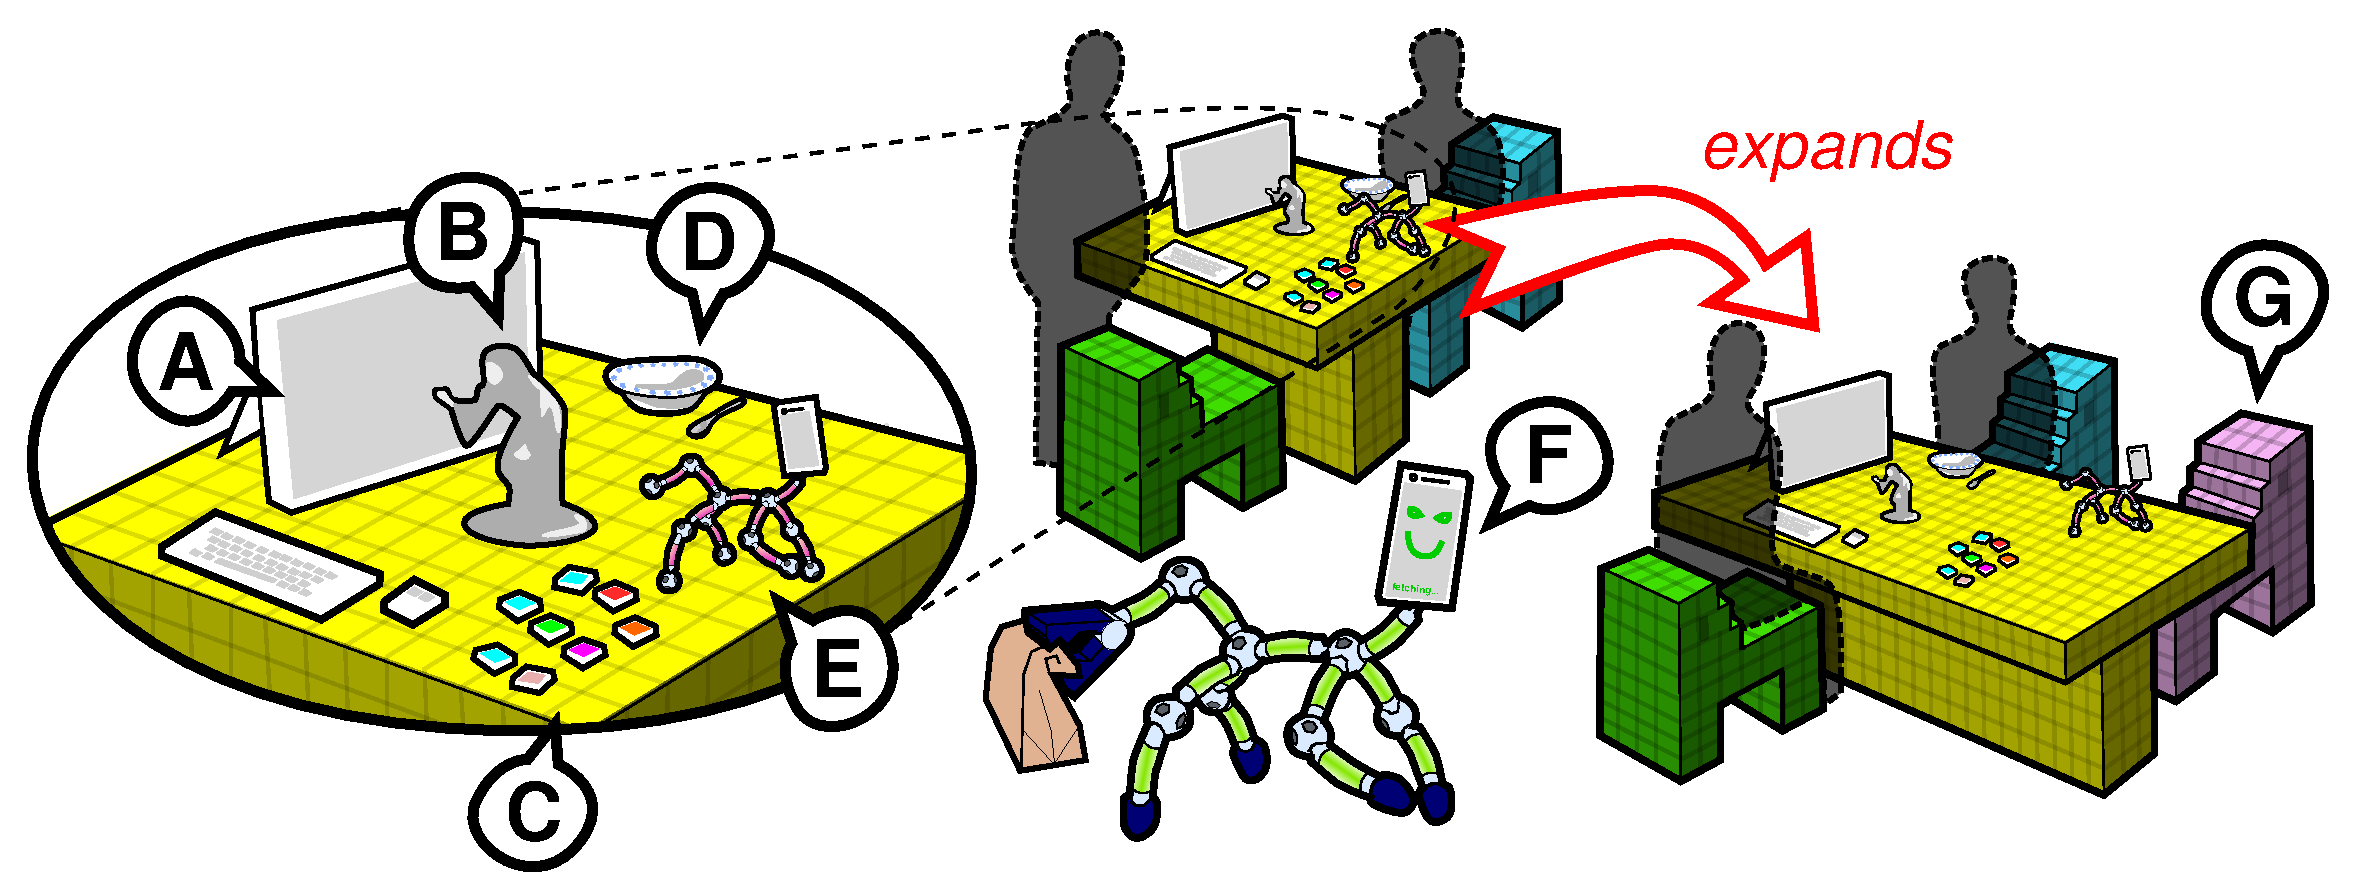
\includegraphics[width=\textwidth]{kinds_of_artifacts.pdf}
    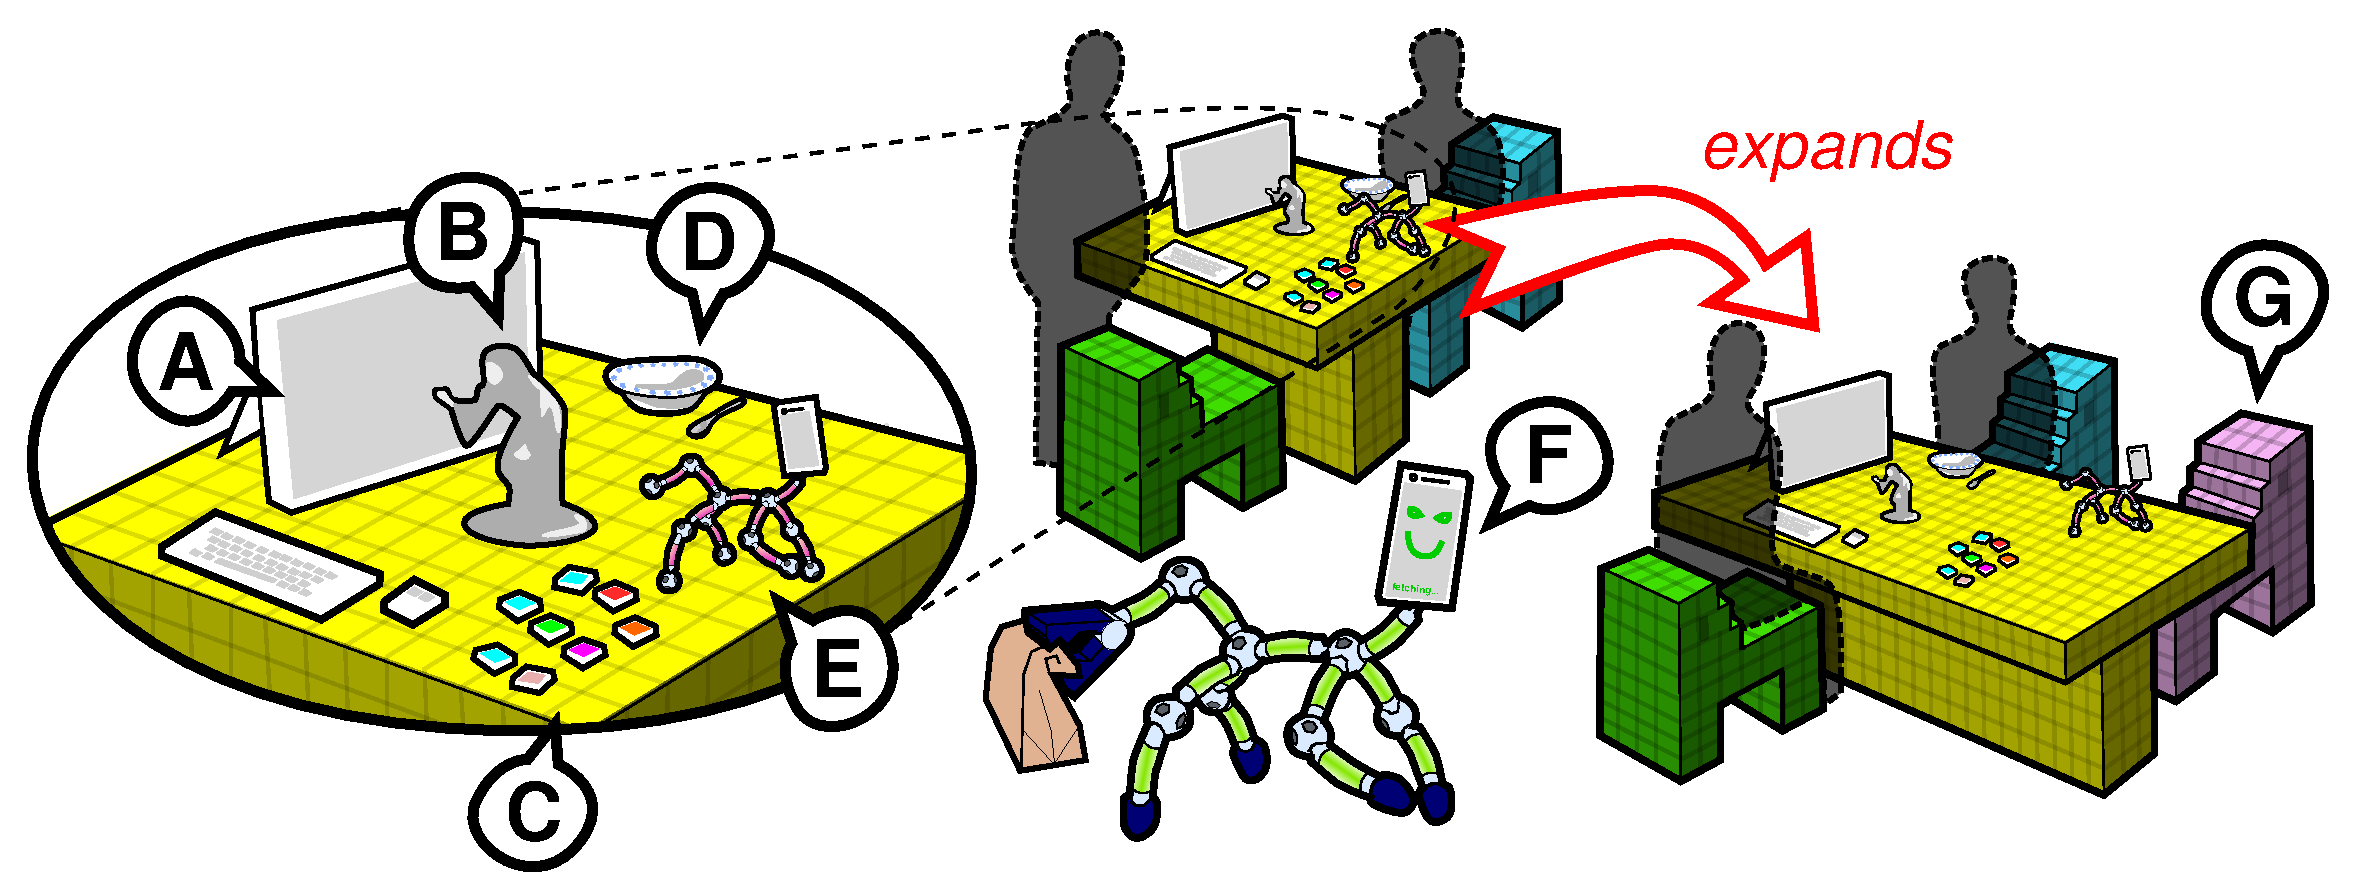
\includegraphics[width=140mm]{kinds_of_artifacts.pdf}
  \caption{An illustration of various kinds of artifacts found in responsive environments: \textbf{\emph{A}} a (work)bench computer (a popsicle); \textbf{\emph{B}} an avatar hyperthou; \textbf{\emph{C}} a tile tinkit; \textbf{\emph{D}} a bowl and spoon (duckcicles); \textbf{\emph{E}} a stickpuppet fig (with a hub-and-strut tinkit body and a volticle crystal for a head); \textbf{\emph{F}} a golem fig fetching lunch; \textbf{\emph{G}} a social table hyperfig (composed of prismatic cube bunkles).}
  \label{fig:kinds_of_artifacts}
\end{figure}

\subsubsection{Sticks}
While many devices in a responsive environment may operate autonomously, it will often be desirable for people to give direct input to control a device. 
We call a device that facilitates realtime control input a `stick', after the classic video game input device the joystick. 

There are several varieties of sticks. 
For example a device that gathers together several buttons and directional controls such as a game controller, or an aerial drone sockpuppet's dedicated control panel, is a \emph{stickboard}. 
The smaller fetchbot model (built with a tinkit) shown in Figure~\ref{fig:kinds_of_artifacts} at \emph{E} could be used as a \emph{stickpuppet} to directly pose the fetchbot golem shown at \emph{F}. 
More nuanced input could be gathered from a partial%
\footnote{For example the g-speak system \citep{gstalt} uses motion capture to identify hand gestures made while wearing special gloves in a space populated with high-resolution video cameras.}
or full-body%
\footnote{For example with a Kinect, an inexpensive system (sold as a peripheral for the XBox video game console) that captures both a depth mapping (using an infrared laser and sensor) and a video stream. This data can be combined to reconstruct a person's full-body pose.}
\emph{sticksuit} that uses either an instrumented space or integrated sensors in clothing (or both) to capture human movement with high fidelity.

\subsubsection{Badges}
While people are adept at visually identifying artifacts and other people, most computational systems need a hint. Badges are devices that can be attached to an artifact or worn by a person to facilitate their identification by responsive devices. Passive badges such as \textbf{QR codes} and \textbf{RFID tags} need to be scanned by a sensor, while active badges such as crystals generally track their own position%
\footnote{Using the \textbf{global positioning system (GPS)} or radio triangulation from known cell towers and wi-fi access points.}
and broadcast it over the network.


\section{Roles for Responsive Environments}
\label{sec:roles}
%
One of the most important aspects of an artifact ecology are the roles available for people to relate to the artifacts within it. In some ecologies only a select few highly trained professionals have any input on the behavior of devices, while other ecologies provide opportunities for a broader spectrum of society to participate. We will not discuss the role a `user' of a locked-down device plays, but only roles that allow some level of input back into the larger ecology.

The roles described here are not meant to define individual people, but rather are different stances that a single person could take toward an artifact at different times. For example a researcher that designs prismatic cube bunkles could also take on the role of a fig designer and create a social table hyperfig. And then later at home the same person could eat dinner at a social table and write up an evaluation of the experience.

The roles are also not separated by discipline (e.g. electrical, mechanical, code) but by level of accessibility. This reflects the ideal of open hardware design that a single person can have an idea for a device and build a prototype to demonstrate it. Spoke and robunculi ecologies attempt to support this development model by packaging the more technologically demanding features in reusable modules. And our organization of roles reflects the reality that modules often span these disciplinary boundaries. (For example the Arduino project packages both electrical and software components, and many of its extension modules include mechanical, electrical and software bits.)

\subsection{Taster}
A person adopting this role, for example a person sitting down at a social table, is relatively passive in relation to the artifact in question. Tasters participate in the ecology by providing critical feedback in relevant forums. This could be as simple as having a specialized gesture expressing approval (or disapproval) of a given hyperfig that is then incorporated into rankings on the online hyperfig repository, or as involved as filing a bug report.

While even in a popsicle ecology journalists and bloggers can play this role, the online design repositories of spoke and robunculi ecologies provide an opportunity for tasters' feedback to be used as debugging data and a filter for identifying successful systems. 

\subsection{Wrangler}
Many devices require substantial input from a person, for example many military sockpuppet drones are operated remotely by a trained pilot at a stickboard. While adopting the roles described below requires some kind of expertise in customizing or building devices, wrangling demands expertise at piloting or otherwise managing devices' behavior in real time.

As wranglers possess a unique perpsective on the behavior of the devices they wrangle, it would be desirable for ecologies to also attract wranglers to serve in design roles. Tinker roles in particular (discussed below) offer an opportunity for wranglers to give design input without a great deal of investment in training.

\subsection{Tinker}
Many people are motivated to understand more about the mechanisms underlying the behavior of responsive devices but lack the technical knowledge required to address systems at the same level as their designers. 
A strategy for engaging this community is to create devices with tink interfaces. 
An example is a golem robunculi kit with instructions for building a given golem that can then be varied, much like lego kits come with instructions that can serve as a jumping-off point for more creative endeavors. 
And while such mechanical tinkering is straightforward, tangible interfaces can also be used to allow tinkering with algorithms%
\footnote{For example Scratch \citep{scratch} has established a model for a visual, fault tolerant tinkering-style programming interface that involves shuffling puzzle-piece chunks of code, although it is screen-based. 
Tern \citep{tern_classroom} applies similar ideas with a tangible interface composed of literal wooden puzzle pieces. 
With Cubelets (nee RoBlocks) \citep{roblocks} a fig specifies both mechanical and algorithmic properties at once.} 
and electronics%
\footnote{For example littleBits \citep{littlebits} package electronic components to afford tinkering with circuits.}.

By providing opportunities for people to tinker with their devices robunculi ecologies can help to both engage people in a conversation about their devices, and recruit people to expand their technological capabilites so that they are able to adopt more technologically demanding roles. By providing places for people to expand and apply their skills, a spoke ecology and its associated hackerspaces can help these new recruits find productive technical roles to play.

\subsection{Tek}
Here we have reached the realm of the professional designer (and engineer). A tek is a person who comes up with ideas for and builds new devices. 
While professional designers are traditionally grouped according to their specialized technical discipline, we suggest that such compartmentalization works against a tek's ability to envision and create useful devices. 

In particular, within spoke and robunculi ecologies the availability of modules that package complex technologies lower the barrier to assuming the role of a tek. 
With robunculi kits the distinction between a tinker and a tek is even somewhat blurred, but as we will describe in Chapter~\ref{ch:case_studies} the creation of a device with new behaviors (rather than a variation on an existing device) will generally involve more advanced tools alongside the bunkles themselves, requiring tek-level proficiency.
We predict that the character of these artifact ecologies with a broad community of people able to assume the role of device designers will contrast sharply with popsicle-dominated ecologies where the character and behavior of devices are largely dictated to the community.

\subsection{Tooler}
Much of the growth of the open hardware scene and the spoke ecology comes from people who are thinking not about creating devices, but about the tools that can help teks to create devices. In doing so these people are assuming the role of a tooler. While a tooler may build a literal tool, such as a 3D printer, they also focus on packaging technologies in modules that make them more accessible. This is common practice in software development (even in popsicle ecologies) and is quickly spreading to electronic and mechanical development in spoke and robunculi ecologies. Again, toolers are not generally defined by discipline as many modules package components from several disciplines. In robunculi ecologies toolers design the bunkles (and their control algorithms) that teks and tinkers use to create devices.

\subsection{Wiz}
Because of the complexity of the technologies involved in creating responsive artifacts, at some point there is a demand for specialization. 
We call someone who considers the deep issues of a discipline, either to extend what can be done, or to make its capabilities more accessible, a wiz.
In adopting the role of a wiz a person could be developing a new programming language, designing a computer chip, developing a new actuator, or creating a new rapid fabrication technology. 
While people able to play such a role are generally prized in any artifact ecology, we suggest that expanding the community of teks has the potential to develop a greater number of wizs, thus advancing the capabilities of the entire ecology.

\section{Examples of Artifact Ecologies}
\label{sec:artifact_ecologies}
%
\subsection{nodes of power}
        \begin{enumerate}
            \item manufacturing
            \item data transmission
            \item data stores
            \item shrines (high-powered computing clusters)
            \item leaf node control
        \end{enumerate}        


\section{Robunculi: an Ontology}
\label{sec:robunculi_ontology}
    \begin{enumerate}
        \item robunculi typologies
        \begin{enumerate}
            \item idols
            \item tangible sketches
            \item golems
            \begin{enumerate}
                \item sock puppet (dumb rc golem)
                \item avatar (golem serving as interface to idol)
            \end{enumerate}
            \item hyperforms
        \end{enumerate}
        \item morphologies
        \begin{enumerate}
            \item tile
            \item block
            \item skeleton (graph)
            \item panel
            \item glass (screen / projection interface)
            \item shrine (idol-scale computing facility)
        \end{enumerate}
        \item affordances
        \begin{enumerate}
            \item parallel affordances are synergistic
            \item placing / self-reconfiguring
            \item posing / flexing (self-posing)
            \item commanding (pointing) / signalling (haloing)
            \item listening (tagging) / responding (texting)
            \item graffing (accepting drawings) / gramming (responding with drawings)
            \item puppeteering / puppeting (present puppeteering interface)
            \item sinks generate structured data to be accessed through idols
            \item logging (recording interactions to data stores) (sink)
            \item crawling (indexing data stores) (sink)
            \item tracking (id-ing and classifying agents with sensors) (sink)
            \item slamming (exploring and mapping environments) (sink)
        \end{enumerate}
    \end{enumerate}






